\section{Gray\-Image\-Data Class Reference}
\label{class_c_s_image_viewer_1_1_gray_image_data}\index{CSImageViewer::GrayImageData@{CSImageViewer::GrayImageData}}
Class containing the actual pixel data for a gray image (one value per pixel).  


Inheritance diagram for Gray\-Image\-Data::\begin{figure}[H]
\begin{center}
\leavevmode
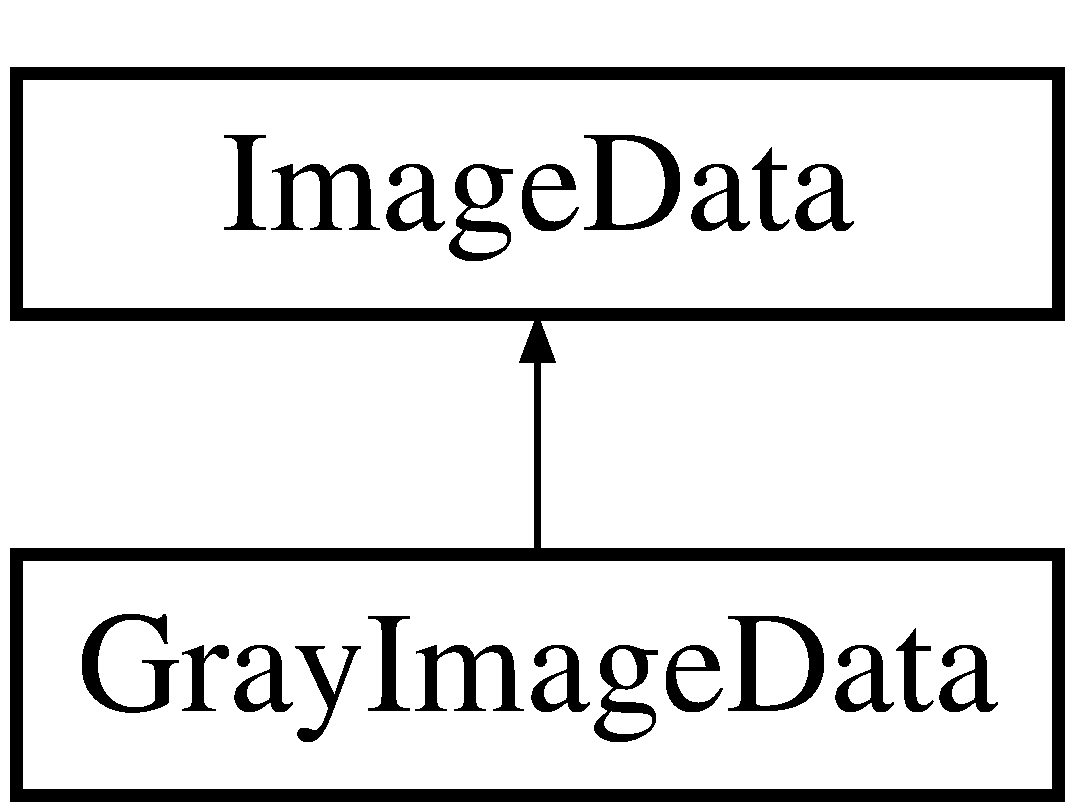
\includegraphics[height=2cm]{class_c_s_image_viewer_1_1_gray_image_data}
\end{center}
\end{figure}
\subsection*{Public Member Functions}
\begin{CompactItemize}
\item 
{\bf Gray\-Image\-Data} (int[$\,$] unpacked, int w, int h)
\begin{CompactList}\small\item\em This ctor constructs a {\bf Gray\-Image\-Data}{\rm (p.\,\pageref{class_c_s_image_viewer_1_1_gray_image_data})} object from an array of gray pixel values and the width and height of the image. m\-Original\-Data will be allocated and set to the pixel values in unpacked. \item\end{CompactList}\item 
{\bf Gray\-Image\-Data} (Bitmap old\-BM, Color[$\,$] old\-Palette, int bpp)
\begin{CompactList}\small\item\em Given a bitmap image and a palette (i.e., color lookup table used to translate scalar image values into other scalar gray values), this ctor reads the image data, uses the lookup table to store the pixel data in an array, and creates a displayable version of the image. m\-Original\-Data will be allocated and set to the pixel values in the bitmap. \item\end{CompactList}\item 
void {\bf unpacked\_\-gray\_\-to\_\-display} (int[$\,$] unpacked)
\begin{CompactList}\small\item\em This function takes an unpacked int array of gray pixel values (representing an entire image), and copies the values to m\-Display\-Data (also representing an entire image). m\-Display\-Image is changed to these values as well. m\-Original\-Data remains unchanged. Note that unpacked must be the same size as the original image (m\-W$\ast$m\-H). \item\end{CompactList}\item 
int {\bf get\-Gray} (int row, int col)
\begin{CompactList}\small\item\em Given a pixel's row and column location, this function returns the gray pixel value. \item\end{CompactList}\end{CompactItemize}


\subsection{Detailed Description}
Class containing the actual pixel data for a gray image (one value per pixel). 



\subsection{Constructor \& Destructor Documentation}
\index{CSImageViewer::GrayImageData@{CSImage\-Viewer::Gray\-Image\-Data}!GrayImageData@{GrayImageData}}
\index{GrayImageData@{GrayImageData}!CSImageViewer::GrayImageData@{CSImage\-Viewer::Gray\-Image\-Data}}
\subsubsection{\setlength{\rightskip}{0pt plus 5cm}{\bf Gray\-Image\-Data} (int[$\,$] {\em unpacked}, int {\em w}, int {\em h})}\label{class_c_s_image_viewer_1_1_gray_image_data_460f31ea25606440ef9dce2e35c2e476}


This ctor constructs a {\bf Gray\-Image\-Data}{\rm (p.\,\pageref{class_c_s_image_viewer_1_1_gray_image_data})} object from an array of gray pixel values and the width and height of the image. m\-Original\-Data will be allocated and set to the pixel values in unpacked. 

\begin{Desc}
\item[Parameters:]
\begin{description}
\item[{\em unpacked}]unpacked array of gray values \item[{\em w}]image width \item[{\em h}]image height \end{description}
\end{Desc}
\begin{Desc}
\item[Returns:]nothing (ctor) \end{Desc}
\index{CSImageViewer::GrayImageData@{CSImage\-Viewer::Gray\-Image\-Data}!GrayImageData@{GrayImageData}}
\index{GrayImageData@{GrayImageData}!CSImageViewer::GrayImageData@{CSImage\-Viewer::Gray\-Image\-Data}}
\subsubsection{\setlength{\rightskip}{0pt plus 5cm}{\bf Gray\-Image\-Data} (Bitmap {\em old\-BM}, Color[$\,$] {\em old\-Palette}, int {\em bpp})}\label{class_c_s_image_viewer_1_1_gray_image_data_148bcda539e1b1a85e03ca8e8c5c595d}


Given a bitmap image and a palette (i.e., color lookup table used to translate scalar image values into other scalar gray values), this ctor reads the image data, uses the lookup table to store the pixel data in an array, and creates a displayable version of the image. m\-Original\-Data will be allocated and set to the pixel values in the bitmap. 

\begin{Desc}
\item[Parameters:]
\begin{description}
\item[{\em old\-BM}]bitmap image used to construct an instance of this class \item[{\em old\-Palette}]color lookup table \item[{\em bpp}]bits-per-pixel \end{description}
\end{Desc}
\begin{Desc}
\item[Returns:]nothing (ctor) \end{Desc}


\subsection{Member Function Documentation}
\index{CSImageViewer::GrayImageData@{CSImage\-Viewer::Gray\-Image\-Data}!getGray@{getGray}}
\index{getGray@{getGray}!CSImageViewer::GrayImageData@{CSImage\-Viewer::Gray\-Image\-Data}}
\subsubsection{\setlength{\rightskip}{0pt plus 5cm}int get\-Gray (int {\em row}, int {\em col})}\label{class_c_s_image_viewer_1_1_gray_image_data_dcb7178c700e5ead72cd80cf91d05c2e}


Given a pixel's row and column location, this function returns the gray pixel value. 

\begin{Desc}
\item[Parameters:]
\begin{description}
\item[{\em row}]image row \item[{\em col}]image column \end{description}
\end{Desc}
\begin{Desc}
\item[Returns:]the gray pixel value at that position.\end{Desc}
\begin{Desc}
\item[{\bf Todo}]project: speed up indexing \end{Desc}
\index{CSImageViewer::GrayImageData@{CSImage\-Viewer::Gray\-Image\-Data}!unpacked_gray_to_display@{unpacked\_\-gray\_\-to\_\-display}}
\index{unpacked_gray_to_display@{unpacked\_\-gray\_\-to\_\-display}!CSImageViewer::GrayImageData@{CSImage\-Viewer::Gray\-Image\-Data}}
\subsubsection{\setlength{\rightskip}{0pt plus 5cm}void unpacked\_\-gray\_\-to\_\-display (int[$\,$] {\em unpacked})}\label{class_c_s_image_viewer_1_1_gray_image_data_2151cfeeab0ceee3eacce0d83a906054}


This function takes an unpacked int array of gray pixel values (representing an entire image), and copies the values to m\-Display\-Data (also representing an entire image). m\-Display\-Image is changed to these values as well. m\-Original\-Data remains unchanged. Note that unpacked must be the same size as the original image (m\-W$\ast$m\-H). 

\begin{Desc}
\item[Parameters:]
\begin{description}
\item[{\em unpacked}]unpacked int array of gray values (all values must be in [0..255]\begin{itemize}
\item no scaling will occur in this function\item only the least significant 8 bits will be used) \end{itemize}
\end{description}
\end{Desc}
\begin{Desc}
\item[Returns:]nothing (void) \end{Desc}


The documentation for this class was generated from the following file:\begin{CompactItemize}
\item 
{\bf Gray\-Image\-Data.cs}\end{CompactItemize}
